% --------------------- VARIABLEN -------------------------

\newcommand{\COURSE}{Physik und Materialwissenschaften\\ Praktikum Physik \\}
\newcommand{\SEMESTER}{Elektro- und Informationstechnik II}
\newcommand{\STUDENT}{Maximilian Spahn\\ und\\Benjamin Langer}

\newcommand{\HEADDING}{Praktikum Physik}
\newcommand{\SUBHEADDING}{Versuch 5.3: Prismenspektroskopie}

% ------------------- DEFINITIONEN -----------------------

\documentclass[a4paper]{scrartcl}

\usepackage[utf8]{inputenc}
\usepackage[ngerman]{babel}
\usepackage{amsmath}
\usepackage{amssymb}
\usepackage{color}
\usepackage{tikz}
\usepackage{float}
\usetikzlibrary{arrows,decorations.markings}
\usepackage{tabularx}
\usepackage{fancybox}
\usepackage{pgfplots}
\usepackage[colorlinks=false,linkcolor=black,urlcolor=blue,bookmarks,bookmarksopen=true]{hyperref}
\usepackage{geometry}
\usepackage{fancyhdr}
\usepackage{subcaption}

\usepackage[page]{totalcount}

%Größe der Ränder setzen
\geometry{a4paper,left=2cm, right=2cm, top=3cm, bottom=2cm, headheight=8cm}

%Kopf- und Fußzeile
\pagestyle {fancy}
\fancyhf{}
\fancyhead[L]{\STUDENT}
\fancyhead[C]{\COURSE}
\fancyhead[R]{\today}

\fancyfoot[L]{\SEMESTER}
\fancyfoot[C]{}
\fancyfoot[R]{Seite \thepage /\pageref{LastPage}}

%Formatierung der Überschrift, hier nichts ändern
\def\header#1#2{
	\begin{center}
		{\Large #1}\\
		{#2}
	\end{center}
}

\numberwithin{equation}{subsection} 

\nocite{*}
\bibliographystyle{plainurl}

\setlength\parindent{0pt}

% ----------------------- DOCUMENT ---------------------------

\begin{document}

\vspace{10pt}
\header{\HEADDING}{\SUBHEADDING}
	
\tableofcontents
	
\newpage
	
\section{Einleitung}
Der Versuch zur Prismenspektroskopie soll die Brechung elektromagnetischer Wellen an einem Prisma zeigen.
Dafür werden Lichtspektren unterschiedlicher Leuchtdioden untersucht.

\newpage
\section{Theorie}

\newpage
\section{Häusliche Vorarbeit}
\subsection{Wie funktioniert eine LED?}
Eine Leuchtdiode (LED) besteht aus 2 Halbleiterschichten, welche in Durchlassrichtung geschaltet sind.
Durch Anlegen einer Spannung wandern Elektronen von der n-dotierten über den pn-Übergang zur p-dotierten Seite.
Dabei geht das Elektron in das energetisch günstigere Valenzband (höheres Energieniveau) über.
Ein Strom fließt durch die Diode und die aufgebaute Diffusionsspannung wird abgebaut.
Die dadurch freiwerdende Energie wird in Form von Licht (Photon) von der Diode ausgesandt.
Dabei hängt die Wellenlänge des ausgestrahlten Lichtes vom Halbleitermaterial und der Dotierung ab. \cite{leifiled}

\subsection{Warum emittiert eine Gasentladungslampe ein Linienspektrum?}
Die Gasentladung in der Lampe entsteht auf Grund von Ionisationsvorgängen.
Wenn man die an den Elektronen anliegende Spannung erhöht, werden die Elektronen immer schneller zur Anode beschleunigt.
Treffen sie auf ihrem Weg mit Neotronen zusammen, können die Elektronen aus den Atomhüllen herausschlagen (elastischer Stoß) und ionisiert werden.
Wird die anliegende Spannung an der Gasentladungslampe immer weiter erhöht, erlangen die Ladungsträger immer größere kinetische Energie, wodurch der Ionisationsvorgang einsetzt.
Man spricht auch von Stoßionisation.
Die ionisierten Elektronen hinterlassen ein Loch auf ihrer Schale.
Ein Elektron fällt auf ein energieniedrigeres Niveau herunter und sendet Licht in Form eines Photons aus.
Dies geschieht gequantelt, da es nur bestimmte Energieniveaus gibt.
Die entstehenden Emissions-Spektrallinien bilden ein Linienspektrum aus. \cite{leifilampe}

\subsection{Unter welchem Winkel $\theta_1$, $\theta_2$ treten die beiden Wellenlängen aus dem Prisma aus?}
Ein paralleles Bündel von Lichtstrahlen, das die beiden Wellenlängen $\lambda_1 = 450\; nm$ und $\lambda_2 = 650\; nm$ enthält, tritt in ein Prisma mit dem Einfallswinkel $\gamma = 45^\circ$ ein.\\
\quad\\
Brechungsindizes:
\begin{align*}
n(\lambda_1) = 1,643 \\
n(\lambda_2) = 1,617
\end{align*}

\begin{figure}[H]
	%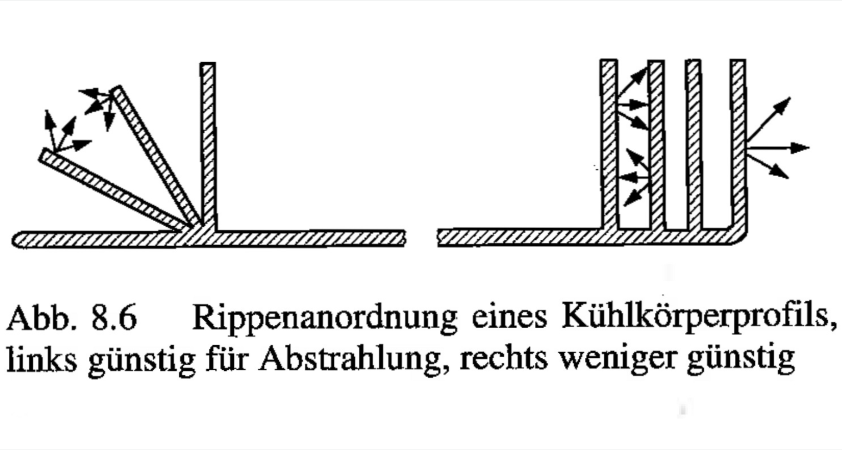
\includegraphics[width=12cm]{Abbildungen/Kuehlkoerper}
	\centering
	\caption{Doppelte Lichtbrechung Prisma}
	\centering
	\label{fig:AufgabePrisma}
\end{figure}

Berechnung von $\theta_1$:
\begin{align*}
	n_{Luft}\sin(\gamma) &= n(\lambda_1)\sin(\alpha_1) \\
	\alpha_1 &= \arcsin\left(\frac{\sin(45^\circ)}{1,643}\right) \\
	\alpha_1 &= 25,49^\circ \\
	\quad \\
	90^\circ - 25,49^\circ &= 64,51^\circ \\
	180^\circ - 60^\circ - 64,51^\circ &= 55,49^\circ \\
	90^\circ - 55,49^\circ &= \beta_1 = 34,51^\circ \\
	\quad \\
	n(\lambda_1)\sin(\beta_1) &= n_{Luft}\sin(\theta_1) \\
	\theta_1 &= \arcsin(1,643^\circ \cdot \sin(34,51^\circ)) \\
	\theta_1 &= 68,57^\circ
\end{align*}

Berechnung von $\theta_2$:
\begin{align*}
	n_{Luft}\sin(\gamma) &= n(\lambda_2)\sin(\alpha_2) \\
	\alpha_2 &= \arcsin\left(\frac{\sin(45^\circ)}{1,617}\right) \\
	\alpha_2 &= 25,93^\circ \\
	\quad \\
	90^\circ - 25,93^\circ &= 64,07^\circ \\
	180^\circ - 60^\circ - 64,07^\circ &= 55,93^\circ \\
	90^\circ - 55,93^\circ &= \beta_2 = 34,07^\circ \\
	\quad \\
	n(\lambda_2)\sin(\beta_2) &= n_{Luft}\sin(\theta_2) \\
	\theta_2 &= \arcsin(1,617^\circ \cdot \sin(34,07^\circ)) \\
	\theta_2 &= 64,94^\circ
\end{align*}

\subsection{Welches Glas ist für die Verwendung in einem Prismenspektrometer am besten geeignet?}

\newpage
\section{Aufbau und Durchführung}

\newpage
\section{Auswertung Versuch}

\newpage
\section{Wertung/Fazit}

\newpage
\section{Anhang}

\newpage
\section{Literatur}

\label{LastPage}

\end{document}
%%% Local Variables:
%%% mode: latex
%%% TeX-master: t
%%% End:
